% Universidade Federal de Campina Grande
% Modelo de Proposta de Disserta��o de Mestrado em Ciencia da Computacao
%
% Feito por: Ana Cristina Alves de Oliveira
% (cristina@dsc.ufcg.edu.br - orientador: Francisco Brasileiro)
% Fevereiro de 2006

% E necessario o arquivo "algorithm.sty", se for construir algoritmos

% Adaptado por: Leandro Dias da Silva
% (leandrodias@ic.ufal.br - Coordenador do PPGI)
% Junho de 2013

% readaptado por: Ailton Felix, Lucas Lins, Marcelo Oliveira
% (oliveiramc@ic.ufal.br - Coordenador do PPGI)
% em Julho de 2018

% readaptado por: Christiano Rossini Martins Costa
% (christiano.rossini.mc@gmail.com)
% em abril de 2020

\documentclass[
	% -- opções da classe memoir --
	12pt,				% tamanho da fonte
	openright,			% capítulos começam em pág ímpar (insere página vazia caso preciso)
	oneside,			% para impressão em recto e verso. Oposto a oneside
	a4paper,			% tamanho do papel. 
	% -- opções da classe abntex2 --
	%chapter=TITLE,		% títulos de capítulos convertidos em letras maiúsculas
	%section=TITLE,		% títulos de seções convertidos em letras maiúsculas
	%subsection=TITLE,	% títulos de subseções convertidos em letras maiúsculas
	%subsubsection=TITLE,% títulos de subsubseções convertidos em letras maiúsculas
	% -- opções do pacote babel --
	brazil,  			% idioma adicional para hifenização
	french,				% idioma adicional para hifenização
	spanish,			% idioma adicional para hifenização
	english				% o último idioma é o principal do documento
	]{abntex2}

% ---
% Pacotes básicos 
% ---
\usepackage{lmodern}			% Usa a fonte Latin Modern			
\usepackage[T1]{fontenc}		% Selecao de codigos de fonte.
\usepackage[utf8]{inputenc}		% Codificacao do documento (conversão automática dos acentos)
\usepackage{indentfirst}		% Indenta o primeiro parágrafo de cada seção.
\usepackage{color}				% Controle das cores
\usepackage{graphicx}			% Inclusão de gráficos
\usepackage{microtype} 			% para melhorias de justificação
% ---

% ---
% Pacotes de citações
% ---
\usepackage[brazilian,hyperpageref]{backref}	 % Paginas com as citações na bibl
\usepackage[alf]{abntex2cite}	% Citações padrão ABNT

% --- 
% CONFIGURAÇÕES DE PACOTES
% --- 

% ---
% Configurações do pacote backref
% Usado sem a opção hyperpageref de backref
\renewcommand{\backrefpagesname}{Citado na(s) página(s):~}
% Texto padrão antes do número das páginas
\renewcommand{\backref}{}
% Define os textos da citação
\renewcommand*{\backrefalt}[4]{
	\ifcase #1 %
		Nenhuma citação no texto.%
	\or
		Citado na página #2.%
	\else
		Citado #1 vezes nas páginas #2.%
	\fi}%
% ---

% ---
% Informações de dados para CAPA e FOLHA DE ROSTO
% ---
\titulo{On the agreement among developers when detecting code smells aided by decision tree}
\autor{Christiano Rossini Martins Costa}
\local{Maceió}
\data{abril de 2020}
\orientador{Baldoino Fonseca dos Santos Neto}
%\coorientador{Equipe \abnTeX}
\instituicao{%
  Universidade Federal de Alagoas
  \par
  Instituto de Computação
  \par
  Programa de Pós-Graduação em Informática}
\tipotrabalho{Dissertação de Mestrado}
% O preambulo deve conter o tipo do trabalho, o objetivo, 
% o nome da instituição e a área de concentração 
\preambulo{Dissertação apresentada como requisito parcial para obtenção do grau de Mestre pelo Curso de Mestrado em Informática do Instituto de Computação da Universidade Federal de Alagoas.}
% ---

% ---
% Configurações de aparência do PDF final

% alterando o aspecto da cor azul
\definecolor{blue}{RGB}{41,5,195}

% informações do PDF
\makeatletter
\hypersetup{
     	%pagebackref=true,
		pdftitle={\@title}, 
		pdfauthor={\@author},
    	pdfsubject={\imprimirpreambulo},
	    pdfcreator={LaTeX with abnTeX2},
		pdfkeywords={abnt}{latex}{abntex}{abntex2}{trabalho acadêmico}, 
		colorlinks=true,       		% false: boxed links; true: colored links
    	linkcolor=blue,          	% color of internal links
    	citecolor=blue,        		% color of links to bibliography
    	filecolor=magenta,      		% color of file links
		urlcolor=blue,
		bookmarksdepth=4
}
\makeatother
% --- 

% ---
% Posiciona figuras e tabelas no topo da página quando adicionadas sozinhas
% em um página em branco. Ver https://github.com/abntex/abntex2/issues/170
\makeatletter
\setlength{\@fptop}{5pt} % Set distance from top of page to first float
\makeatother
% ---

% ---
% Possibilita criação de Quadros e Lista de quadros.
% Ver https://github.com/abntex/abntex2/issues/176
%
\newcommand{\quadroname}{Quadro}
\newcommand{\listofquadrosname}{Lista de quadros}

\newfloat[chapter]{quadro}{loq}{\quadroname}
\newlistof{listofquadros}{loq}{\listofquadrosname}
\newlistentry{quadro}{loq}{0}

% configurações para atender às regras da ABNT
\setfloatadjustment{quadro}{\centering}
\counterwithout{quadro}{chapter}
\renewcommand{\cftquadroname}{\quadroname\space} 
\renewcommand*{\cftquadroaftersnum}{\hfill--\hfill}

\setfloatlocations{quadro}{hbtp} % Ver https://github.com/abntex/abntex2/issues/176
% ---

% --- 
% Espaçamentos entre linhas e parágrafos 
% --- 

% O tamanho do parágrafo é dado por:
%\setlength{\parindent}{1.3cm}

% Controle do espaçamento entre um parágrafo e outro:
%\setlength{\parskip}{0.2cm}  % tente também \onelineskip

% ---
% compila o indice
% ---
\makeindex
% ---


% ---
% Pacotes acessórios
% ---
\usepackage{longtable}
\usepackage{tabulary}
\usepackage{tabu}
\usepackage{ltablex}
\usepackage{times}
%\usepackage{fancyhdr}
%\usepackage{fancyvrb}
\usepackage{algorithmic}
\usepackage[nothing]{algorithm}
\usepackage{latexsym}
\usepackage{amsmath}  %texto no modo math
%\usepackage[colorlinks,pdftex,pdfpagelabels=false]{hyperref} % Inclusão de links 
\usepackage{graphicx,url}
\usepackage{import}
\usepackage{booktabs}
\usepackage{lscape}
\usepackage{flushend}
\usepackage[table,xcdraw]{xcolor}
\usepackage{multirow}
\usepackage{color, colortbl}
\usepackage{todonotes}
\usepackage{pdfpages}
%\usepackage{hyperref} % controla a formação do índice
% ---

% ----
% Comandos de estilo e espacamento (Personalização) ----------------------------------------
% ----
% \newlength{\defbaselineskip}
% \setlength{\defbaselineskip}{\baselineskip}
% \newcommand{\setlinespacing}[1]%
%           {\setlength{\baselineskip}{#1 \defbaselineskip}}

% \setcounter{topnumber}{2}
% \renewcommand{\topfraction}{.7}
% \setcounter{bottomnumber}{1}
% \renewcommand{\bottomfraction}{.3}
% \setcounter{totalnumber}{3}
% \renewcommand{\textfraction}{.2}
% \renewcommand{\floatpagefraction}{.5}
% \setcounter{dbltopnumber}{2}
% \renewcommand{\dbltopfraction}{.7}
% \renewcommand{\dblfloatpagefraction}{.5}
% %
% \oddsidemargin -28pt
% \evensidemargin -28pt
% \marginparwidth 50pt
% \marginparsep 5pt
% \topmargin -27pt
% \hoffset 15mm
% \textheight 237mm
% \textwidth 155mm
% \renewcommand{\baselinestretch}{1.5}
% %
% \newenvironment{braced}
%  {\par\smallskip\hbox to\columnwidth\bgroup
%   \hss$\left\{\begin{minipage}{\columnwidth}}
%  {\end{minipage}\right\}$\hss\egroup\smallskip}

% % Color definitions (RGB model)
% \definecolor{mycolor1}{rgb}{0.753,0.753,0.753}

% ----

% ----
% Reestilização dos capítulos ----------------------------------------
% ----
\renewcommand{\ABNTEXchapterfont}{\fontfamily{cmr}\fontseries{b}\selectfont}
\renewcommand{\ABNTEXchapterfontsize}{\HUGE}
% --------------------------------------------------------------------

% ----
% Início do documento
% ----
\begin{document}

% Seleciona o idioma do documento (conforme pacotes do babel)
\selectlanguage{english}
%\selectlanguage{brazil}

% Retira espaço extra obsoleto entre as frases.
\frenchspacing 

% ----------------------------------------------------------
% ELEMENTOS PRÉ-TEXTUAIS
% ----------------------------------------------------------
% \pretextual

% ---
% Capa (versão canônica ABNTEX2)
% ---
%\imprimircapa  
% ---

% ---
% Capa (versão alternativa UFAL)
% ---
\import{sections/}{capa.tex}
\imprimircapa

% ---
% Folha de rosto (versão canônica ABNTEX2)
% (o * indica que haverá a ficha bibliográfica)
% ---
%\imprimirfolhaderosto*
% ---

% ---
% Folha de Rosto (versão alternativa UFAL)
% ---
\import{sections/}{folha-de-rosto.tex}
\imprimirfolhaderosto*

%
% Filha catalográfica
%
\begin{fichacatalografica}
    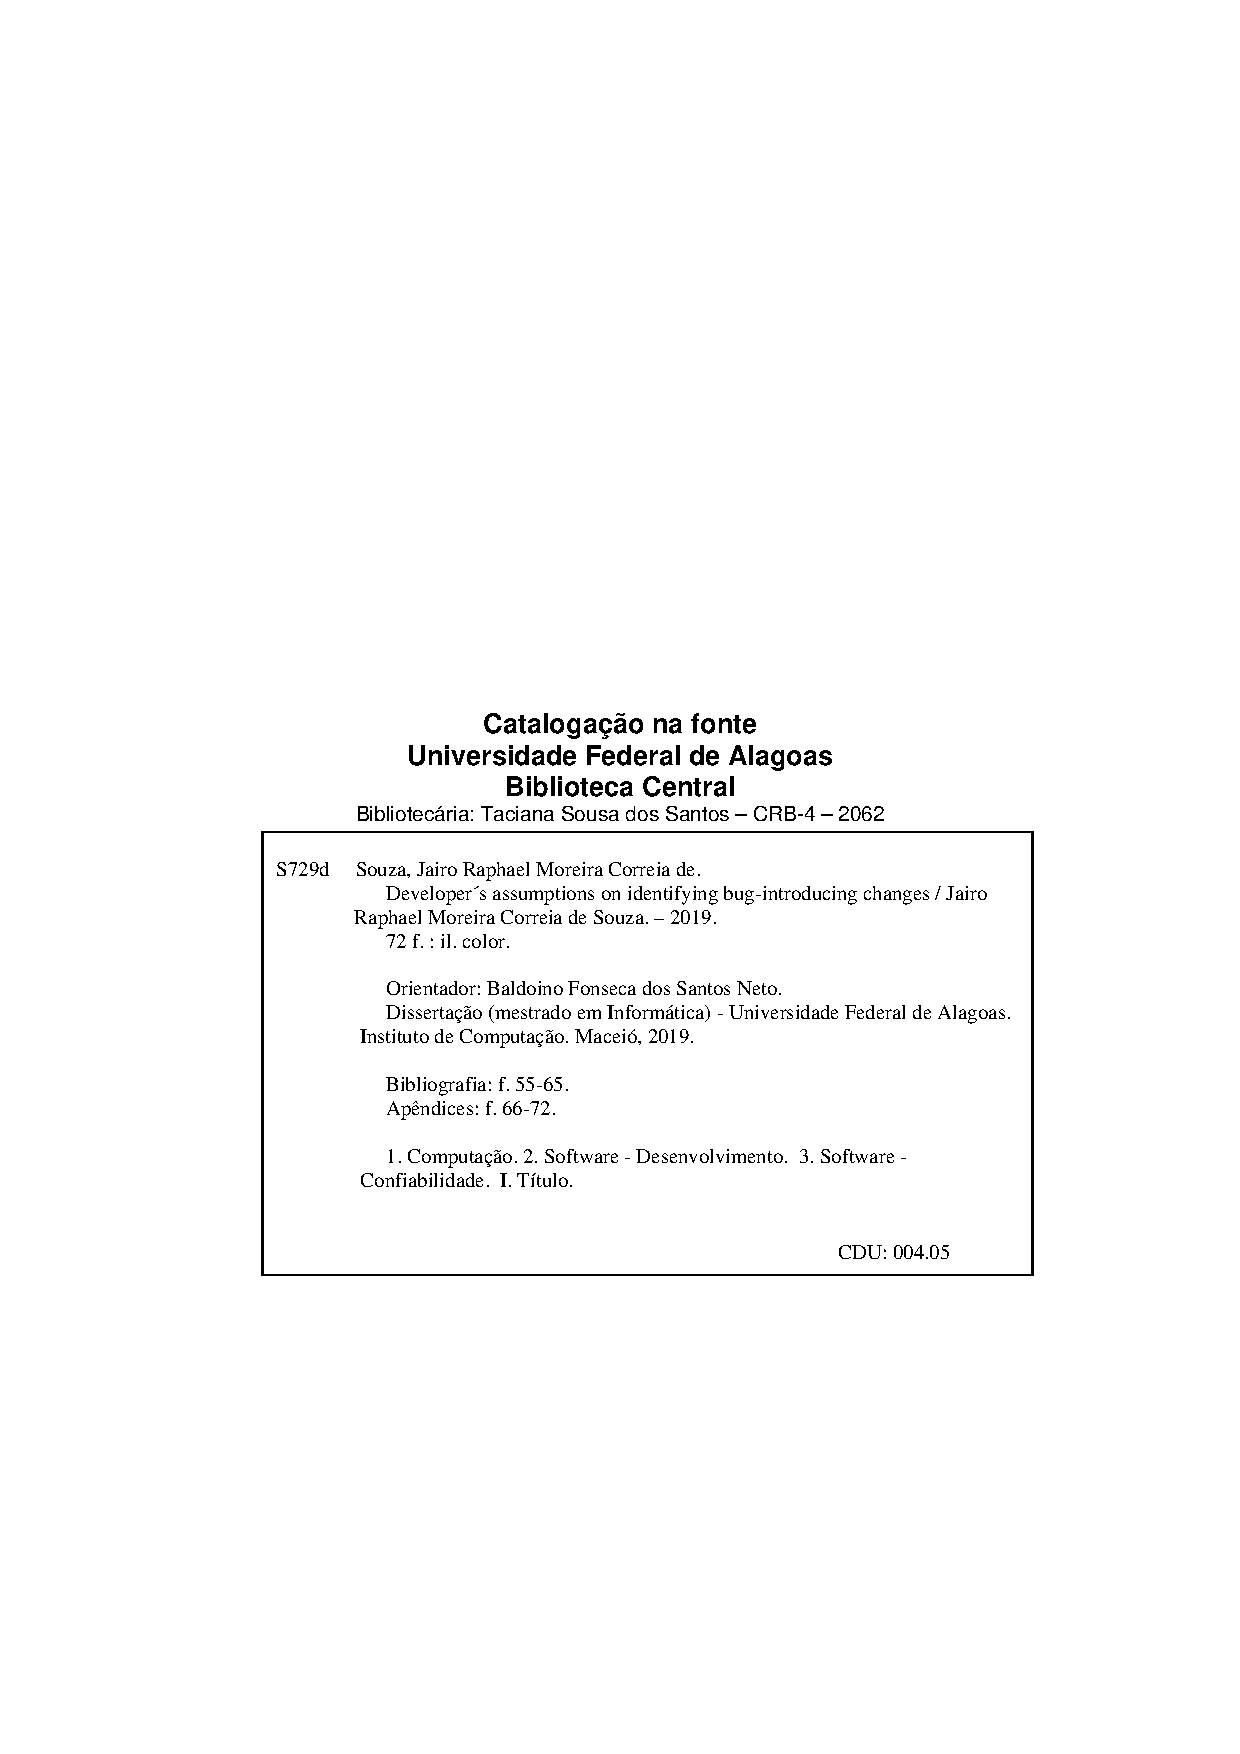
\includepdf[pages=-,pagecommand={}]{Fichacat7910-2019.pdf}
\end{fichacatalografica}
%\import{sections/}{folha-aprovacao.tex}

%
% Folha de aprovação para ser impressa e preenchida pela banca examinadora
%
\begin{folhadeaprovacao}
    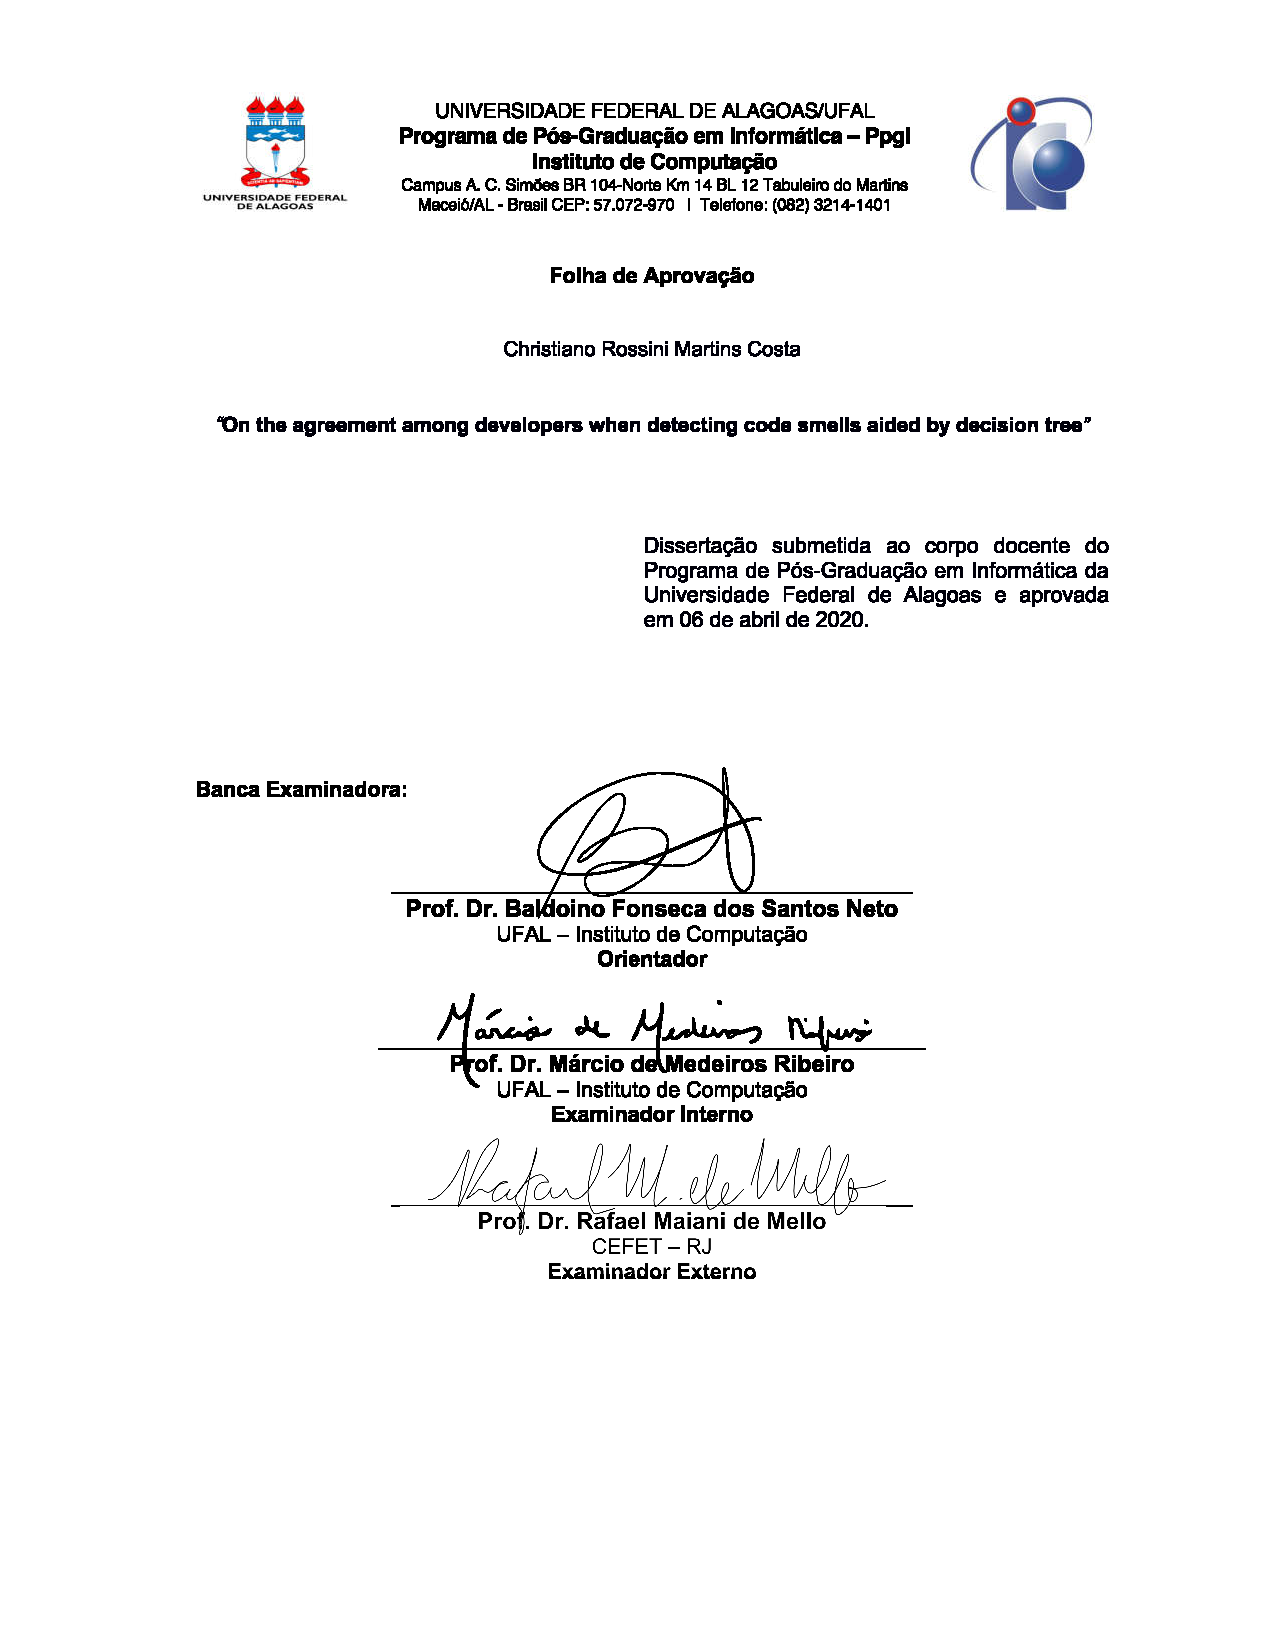
\includepdf[]{folha_aprovacao.pdf}
\end{folhadeaprovacao}

%
% Dedicatória
%
\begin{dedicatoria}
   \vspace*{\fill}
   \centering
   \noindent
   \textit{ Este trabalho é dedicado às crianças adultas que,\\
   quando pequenas, sonharam em se tornar cientistas.} \vspace*{\fill}
\end{dedicatoria}

%
% Agradecimentos
%
\begin{agradecimentos}
    \import{sections/}{agradecimentos.tex}
\end{agradecimentos}
% ---

% ---
% RESUMOS
% ---

% resumo em português
\setlength{\absparsep}{18pt} % ajusta o espaçamento dos parágrafos do resumo
\import{sections/}{resumo.tex}

% resumo em inglês
\import{sections/}{abstract.tex}
% ---

% ---
% inserir lista de ilustrações
% ---
\pdfbookmark[0]{\listfigurename}{lof}
\listoffigures*
\cleardoublepage
% ---

% ---
% inserir lista de tabelas
% ---
\pdfbookmark[0]{\listtablename}{lot}
\listoftables*
\cleardoublepage
% ---

% ---
% inserir o sumario
% ---
\pdfbookmark[0]{\contentsname}{toc}
\tableofcontents*
\cleardoublepage
% ---


% ----------------------------------------------------------
% ELEMENTOS TEXTUAIS
% ----------------------------------------------------------
\textual

% ---
% Introdução
% ---
\import{sections/}{01-introduction.tex}
% ---
% Fundamentação teórica
% ---
\import{sections/}{02-background.tex}
% ---
% Design de pesquisa
% ---
\import{sections/}{03-study-design.tex}
% ---
% Resultados
% ---
\import{sections/}{04-results.tex}
% ---
% Discussões
% ---
\import{sections/}{05-discussions.tex}
% ---
% Trabalhos relacionados
% ---
\import{sections/}{06-related-work.tex}
% ---
% Ameaças à validade
% ---
\import{sections/}{07-threats.tex}
% ---
% Conclusão
% ---
\import{sections/}{08-conclusion.tex}
% ---


% ----------------------------------------------------------
% ELEMENTOS PÓS-TEXTUAIS
% ----------------------------------------------------------
\postextual
% ----------------------------------------------------------

% ----------------------------------------------------------
% Referências bibliográficas
% ----------------------------------------------------------
\bibliography{mybibfile} % arquivos com as entradas bib.


% ----------------------------------------------------------
% Apêndices
% ----------------------------------------------------------
\import{sections/}{09-appendix.tex}


%%%%%%%%%%%%%%%%%%%%%%%%%%%%%%%%%%%%%%%%%%%%%%%%%%%%%%%%%%%%%%%%%%%%%%%%%%%%%%%%


\end{document}